\documentclass{beamer}
\usetheme{tokitex}

\usepackage{graphics}
\usepackage{multirow}
\usepackage{tabto}

\usepackage[english,bahasa]{babel}
\newtranslation[to=bahasa]{Section}{Bagian}
\newtranslation[to=bahasa]{Subsection}{Subbagian}

\usepackage{listings, lstautogobble}
\usepackage{color}

\definecolor{dkgreen}{rgb}{0,0.6,0}
\definecolor{gray}{rgb}{0.5,0.5,0.5}
\definecolor{mauve}{rgb}{0.58,0,0.82}

\lstset{frame=tb,
  language=pascal,
  aboveskip=1mm,
  belowskip=1mm,
  showstringspaces=false,
  columns=fullflexible,
  keepspaces=true,
  basicstyle={\small\ttfamily},
  numbers=none,
  numberstyle=\tiny\color{gray},
  keywordstyle=\color{blue},
  commentstyle=\color{dkgreen},
  stringstyle=\color{mauve},
  breaklines=true,
  breakatwhitespace=true,
  autogobble=true
}

\title{Perkenalan Graph}
\author{Tim Olimpiade Komputer Indonesia}
\date{}

\begin{document}

\begin{frame}
\titlepage
\end{frame}

\begin{frame}
\frametitle{Pendahuluan}

\end{frame}

\begin{frame}
\frametitle{Mengenal Graph}
Graph merupakan struktur data yang terdiri dari \alert{node/vertex} dan \alert{edge}. Node direpresentasikan dengan bentuk lingkaran dan edge direpresentasikan dengan bentuk garis pada ilustrasi dibawah ini.

\begin{figure}
	\centering
	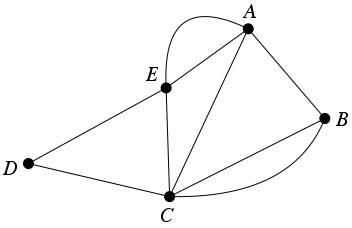
\includegraphics[width=6 cm]{asset/graph.jpg}
\end{figure}
\end{frame}

\begin{frame}
Melalui ilustrasi diatas, dapat disimpulkan bahwa edge bertugas menghubungkan antar-node.  
\end{frame}

\begin{frame}
\frametitle{Jenis Graph}
Berdasarkan hubungan antar node, graph terbagi menjadi 2 :
\begin{itemize}
	\item Directed graph, yaitu graph satu arah. Di graph jenis ini, jika terdapat edge dari A ke B, maka belum tentu terdapat edge dari B ke A. Contoh graph ini adalah kota-kota sebagai nodenya dan jalan 1 arah sebagai edgenya.
	\item Undirected graph, yaitu graph dua arah. Dalam graph ini, jika terdapat edge dari A ke B, maka pasti juga terdapat edge dari B ke A. Contoh graph jenis ini adalah kota-kota sebagai nodenya dan jalan 2 arah sebagai edgenya.
\end{itemize}
Berdasarkan weight dari edgenya, graph juga terbagi menjadi 2 :
\begin{itemize}
	\item Unweighted Graph, yaitu graph dimana edgenya tidak memiliki value, sehingga semua edge memiliki weight 1 dan hanya bermakna bahwa memang terdapat hubungan antar node yang dihubungkannya. 
\end{itemize}
\end{frame}

\end{document}